\chapter{Monadic Parser}

\section{Introduction}

In functional programming, a popular approach to build recursive descent parsers is to model parsers as functions, and to define higher-order functions (or combinators) that implement grammar constructions such as sequencing, choice, and repeatition. Wadler \cite{Wadler:1992} has been realised that using monad, an algebraic structure for mathematics, to build parsers would brings lots practical benefics. For example, using a monadic sequencing combinators for parsers avoids the messy manipulation of nested tuples of results present in earlier work. Moreover, using \textit{monad comprehension} notation makes parser more compact and easy to read.

A monadic parser could be expressed in a modular way in terms of two simpler monads, so that the basic parser combinators no longer need to be defined explicitly. Rather, they arise automatically as a special case of lifting monad operations from a base monad \textit{m} to a certain other monad parameterised over \textit{m}. \cite{Hutton:1996}

Monadic parser combinators makes it easy to write complicated parsers by combining those basic parsers togethers, which makes the parser looks just like the grammer definition in BNF notation. With the benefic of monadic nature, we could easily change the nature of the basic parser monad and the modification will automatically arise to those existing parsers via lifting construction. It highly increases the robustness, flexibility and availability of the library.

This library is built in F2J, which does not supports type classes just like Haskell. So in this library, We used the most basic functions \texttt{bind} and \texttt{result} just for \texttt{Parser[T]} to build monadic parsers. We also provides some useful basic parsers, such as \texttt{char} for parsing one single character, \texttt{string} for parsing a specific sequence of characters, \texttt{choice} and \texttt{many} for choice and repeatition.

We used this parser combinators library for case studies, parsing simple arithmetic expression, XML, Feather Weight Java and a subset grammar of F2J itself. Currently F2J does not support modular compilation, to manage the large code base of the case studies, We wrote a simple script to perform \textit{C-like include} to simulate modular system. To test the parsers above, We wrote a simple test framework in F2J to manage and run test cases automatically.

\section{Project Structure}

The project is hosted on Github (\url{https://github.com/zonyitoo/FParser}) and mirrored in (\url{https://github.com/hkuplg/FParser}). Open source under BSD license.

\begin{lstlisting}[language={}]
.
|-- AUTHORS
|-- LICENSE
|-- Makefile
|-- README.md
`-- src
\end{lstlisting}

The main source code is located under \texttt{src} folder. We also provide a \texttt{Makefile} for building and running the tests, just type \texttt{make test} under the root directory.

\begin{lstlisting}[language={}]
src
|-- Makefile
|-- Makefile.inc
|-- clean                 // Clean the intermediate outputs
|-- eq.sf                 // Definition of Eq[A]
|-- example_arithexpr.sf  // Example of arithmetic expr parser
|-- example_f2j_parser.sf // Example of F2J parser
|-- example_fj_parser.sf  // Example of FWJava parser
|-- example_parser.sf     // Example of basic parsers
|-- example_xml_parser.sf // Example of XML parsers
|-- f2j_parser.sf         // Definition of F2J parser
|-- fj_parser.sf          // Definition of FWJava parser
|-- include.py            // C-like include script
|-- maybe.sf              // Definition of Maybe[A]
|-- order.sf              // Definition of Order
|-- parser.sf             // Definition of basic parsers
|-- plist.sf              // Lazy evaluation ADT list
|-- prelude.sf            // Prelude
|-- pstring.sf            // Definition of PString
|-- result.sf             // Definition of Result[T, E]
|-- run.sh                // Helper script for running test program
|-- show.sf               // Definition of Show[A]
|-- simple_arith_expr_parser.sf // Definition of arithmetic expr parser
|-- test_all.sf           // Run all test cases
|-- test_f2j_parser.sf    // Test cases for F2J parser
|-- test_fj_parser.sf     // Test cases for FWJava parser
|-- test_parser.sf        // Test cases for basic parsers
|-- test_parser_helpers.sf // Helpers for testing parsers
|-- test_plist.sf         // Test cases for lazy ADT list
|-- test_simple_arith_expr_parser.sf // Test arithmetic expr parser
|-- test_xml_parser.sf    // Test cases for XML parser
|-- testfx.sf             // Definition of test framework
|-- thunk.sf              // Definition of Thunk[A]
`-- xml_parser.sf         // Definition of XML parser
\end{lstlisting}

The basic parsers are defined in \texttt{parser.sf}. All the other basic data structures, helper functions and parsers for case studies are defined in their own file. When compiling, you must use \texttt{include.py} to analyse the dependencies and generate a huge combined file, which contains all the depended modules. And let the F2J compiler compile that combined file.

The \texttt{run.sh} script will do the above steps for you and call \texttt{f2j -r} to run the program.

The \texttt{test\_all.sf} is the entrance of running all test cases, you could simply run \texttt{make test} to run all the test cases, or do it manually by \texttt{./run.sh test\_all.sf}.

\section{Parser Core}

The core of parser is defined in \texttt{parser.sf}.

\subsection{Parser Definition}

According to \cite{Hutton:1996}, the parser could be defined as

\begin{lstlisting}
type Parser[T] = String -> [(T, String)];
\end{lstlisting}

Because F2J is call by value, so if we use the builtin List directly, the parser will have very bad performance, because it will try to generate all possible intermediate results but just a few of them are useful for producing the result. So we make a lazy evaluated list \texttt{PList} in \texttt{plist.sf}:

\begin{lstlisting}
data PList[A] = Nil
              | Cons A (Thunk[PList[A]])
              ;
\end{lstlisting}

The \texttt{Thunk} is the key for lazy evaluation, defined in \texttt{thunk.sf}:

\begin{lstlisting}
type Thunk[A] = Unit -> A;
let invoke[A] (t : Thunk[A]) : A =
    t ();
\end{lstlisting}

When we need the rest of the list, just use \texttt{invoke} to enforce evaluation of the rest of the list. So the parser will not parse all intermediate results unless they are required.

Also, the \texttt{String} in F2J is Java's builtin String, which may not suitable for parsing, because lots of \texttt{substring} calls and string concatenation are required while parsing. It would be better if we transform the input to become a linked list of \texttt{Char}. So we also define a type \texttt{PString} in \texttt{pstring.sf}.

\begin{lstlisting}
type PString = PList[Char];
\end{lstlisting}

And then, the parser type in the library is

\begin{lstlisting}
type Parser[T] = PString -> PList[(T, PString)];
\end{lstlisting}

Parsing location is helpful when analysing parse errors, so we have \texttt{SourcePos} containing the position in the input source.

\begin{lstlisting}
type SourceName   = String;
type Line         = Int;
type Column       = Int;

data SourcePos = SourcePos SourceName Line Column;
\end{lstlisting}

And then the parser input and output could carry the position in the source file.

\begin{lstlisting}
type ParseInput = (SourcePos, PString);
type ParseContext[A] = (A, ParseInput);
type ParseOutput[A] = PList[ParseContext[A]];
\end{lstlisting}

The final parser definition is

\begin{lstlisting}
type Parser[A] = ParseInput -> ParseOutput[A];
\end{lstlisting}

\subsection{Primitive Parsers}

For monadic parser combinators, there are two basic parsers: \texttt{result} and \texttt{zero}.

\begin{lstlisting}
let result[V] (value : V) : Parser[V] =
    \(inp : ParseInput) ->
        singleton[ParseContext[V]] (newParseContext[V] value inp);

let zero[V] : Parser[V] =
    \(inp : ParseInput) -> Nil[ParseContext[V]];
\end{lstlisting}

These two basic parsers will construct two monad of parsers. The \texttt{result} will construct a parser which will always returns the \texttt{value} without consuming any inputs as \texttt{[(value, inputString)]}. The \texttt{zero} will construct a parser which will always returns an empty list \texttt{[]} no matter what the input string is.

With these two basic parser, we could build our first parser \texttt{item}, which will takes the first character if the input string is not empty, otherwise it will return an empty output.

\begin{lstlisting}
let item : Parser[Char] =
    \(inp : ParseInput) ->
        case parseInputData inp of
            Nil         ->      Nil[ParseContext[Char]]
          | Cons c xs   ->
                -- Construct the [(c, xs)]
                singleton[ParseContext[Char]]
                    (newParseContext[Char]
                        c
                        (newParseInput
                            (updatePosChar (parseInputPos inp) c)
                            (invoke[PString] xs)));
\end{lstlisting}

It looks compilcated, but actually it is obvious. First it pattern match the input string, if it is empty, then returns empty result, otherwise, take the first character as the parse result, and then put the rest of the input string as the second element of parse output.

\subsection{Parser Combinators}

The primitive parsers are not very useful themselves, we need some helper functions to form more useful parsers.

To implement \textit{monadic} parser combinators, we need two basic monadic operations: \texttt{bind} and \texttt{return}. The \texttt{return} operation is the primitive parser \texttt{result}, then we only need to define the monadic \texttt{bind}:

\begin{lstlisting}
let bind[A, B] (p : Parser[A]) (f : A -> Parser[B]) : Parser[B] =
    \(inp : ParseInput) ->
        concat[ParseContext[B]]
              (map[ParseContext[A], ParseOutput[B]]
                  (\(v : ParseContext[A]) -> f (parseContextResult[A] v) (parseContextInput[A] v)) (p inp));
\end{lstlisting}

It would be easier to understand if we rewrite it in Haskell's list comprehension syntax:

\begin{lstlisting}[language=Haskell]
bind      :: Parser a -> (a -> Parser b) -> Parser b
p `bind` f = \inp -> concat [f v inp’ | (v,inp’) <- p inp]
\end{lstlisting}

The \texttt{bind} is a monadic sequencing combinator, which integrates the sequencing of parsers with the processing of their result values. It would be interpreted as follows. First of all, the parser p is applied to the input string, yielding a list of \texttt{(value, parseInput)} pairs. Now since \texttt{f} is a function that takes a value and returns a parser, it can be applied to each value in order. This results in a list of lists of \texttt{(value, parseInput)} pairs, that can then be flattened to a single list using \texttt{concat}.

The \texttt{bind} combinator avoids the problem of nested tuples of result because the results of the first parser are made directly available for processing by the second, rather than being paired up with the other results to be processed later on.

In BNF notation, the large grammer is built from smaller grammers using a \textit{sequencing} operator -- denoted by juxtaposition, and a \textit{choice} operator -- denoted by a vertical bar \texttt{|}.

To define a \textit{sequencing} operator, we will have a \texttt{seq} combinator:

\begin{lstlisting}
let seq[A, B] (p : Parser[A]) (q : Parser[B]) : Parser[(A, B)] =
    bind[A, (A, B)] p (\(x : A) ->
    bind[B, (A, B)] q (\(y : B) ->
    result[(A, B)] (x, y)));
\end{lstlisting}

The \texttt{seq} combinator will applies one parser after the other, with the result from the two parser being combined as pairs. This parser may leads to parsers with nested tuples as results, which are messy to manipulate. As you can see in the above, \texttt{seq} is equivalent to two \texttt{bind} operations, and you could apply some basic transformations in the last closure, which avoids the nested pairs. So the \texttt{seq} is not very useful in the library, but still provided in case of some special usages.

For \textit{choice} operator, we could define a \texttt{choice} combinator:

\begin{lstlisting}
let choice[A] (p : Parser[A]) (q : Parser[A]) : Parser[A] =
    \(inp : ParseInput) ->
        (p inp) ++[ParseContext[A]] (q inp);
\end{lstlisting}

The \texttt{choice} combinator will concatenate the two parses' results into one. But this combinator could be optimized, because most of the time, we only needs some of the results of the parser \texttt{p}, but this combinator will actually let parser \texttt{q} computes at least one of its results. To make use of the lazy evaluation list nature, \texttt{choice} could be modified as follows:

\begin{lstlisting}
let choice[A] (p : Parser[A]) (q : Parser[A]) : Parser[A] =
    \(inp : ParseInput) ->
        (p inp) +~[ParseContext[A]] (\(__ : Unit) -> q inp);
\end{lstlisting}

The operator \texttt{+\textasciitilde{}} is the lazy version of \texttt{++}, it accepts a thunk as the second parameter, so that it could delay the computation of \texttt{q inp}.

We already has a primitive parser \texttt{item}, which will consumes one character unconditionally. With the power of bind, in practice, we could build a parser which could consumes a certain specific character, \texttt{sat} parser. The \texttt{sat} parser takes a predicate (a function takes a character as parameter and return a boolean value), and returns a parser that consumes one single character if it \textit{satisfies} the predicate, or fails otherwise:

\begin{lstlisting}
let sat (f : Char -> Bool) : Parser[Char] =
    bind[Char, Char] item (\(x : Char) ->
        if f x then
            (result[Char] x)
        else
            zero[Char]);
\end{lstlisting}

Using \texttt{sat}, we can define parsers for specific characters, single digits, lower-case letters and upper-case letters:

\begin{lstlisting}
let char (x : Char) : Parser[Char] =
    sat (\(y : Char) -> x `charEq` y);

let notchar (x : Char) : Parser[Char] =
    sat (\(y : Char) -> x != y);

let digit : Parser[Char] =
    sat (\(x : Char) -> java.lang.Character.isDigit(x));

let upper : Parser[Char] =
    sat (\(x : Char) -> java.lang.Character.isUpperCase(x));

let lower : Parser[Char] =
    sat (\(x : Char) -> java.lang.Character.isLowerCase(x));
\end{lstlisting}

For example, if we apply the parser \texttt{char 'F'} to the input string \texttt{"FCore To Java"}, it will succeeds with a single successful result \texttt{[('F', "Core To Java")]}, since the parser \texttt{char 'F'} succeeds with the character \texttt{'F'}. On the other hand, apply the parser \texttt{lower} to the string \texttt{"FCore to Java"} will fail with an empty result \texttt{[]}, since the character \texttt{'F'} is not a lower-case character.

With \texttt{digit}, \texttt{upper} and \texttt{lower}, we could have some parsers for more practical usage:

\begin{lstlisting}
let letter : Parser[Char] =
    choice[Char] lower upper;

let alphanum : Parser[Char] =
    choice[Char] letter digit;

let noneof (s : String) : Parser[Char] =
    sat (\(x : Char) -> (charin x (pStringFromString s)) `boolEq` False);

let oneof (s : String) : Parser[Char] =
    sat (\(x : Char) -> (charin x (pStringFromString s)));
\end{lstlisting}

The \texttt{letter} parser will parse one character in lower-case and upper-case, and the \texttt{alphanum} will parse one letter and digital character. Moreover, \texttt{noneof} takes an String (a list of characters) and yields a parser that will parse one single character that is not in the provided String, in contract, \texttt{oneof} will yields a parser that will parse one single character that is in the provided String.

Operators could provide more convenience to write parsers, such that if we use the function \texttt{bind} in infix notation \texttt{p `bind` f}, and define an operator \texttt{>>=} works just like \texttt{bind}, and then it could be writtern as \texttt{p >>= f}, which is more obvious and easy to read.

\begin{lstlisting}
let (>>=)[A, B] (p : Parser[A]) (f : A -> Parser[B]) : Parser[B] =
    bind[A, B] p f;

let (>>)[A, B] (p : Parser[A]) (q : Parser[B]) : Parser[B] =
    p >>=[A, B] (\(__ : A) -> q);

let (<*)[A, B] (p : Parser[A]) (q : Parser[B]) : Parser[A] =
    p >>=[A, A] (\(a : A) ->
    q >>=[B, A] (\(__ : B) ->
    result[A] a));
\end{lstlisting}

The operators \texttt{>>} and \texttt{<*} are the special versions of \texttt{bind}. The \texttt{>>} will discard the result of the first parser and return the result of the second parser, while the \texttt{<*} will discard the second one.

If we want to manipulate the result of one parser, we could provide a helpful combinator \texttt{using}, which will take a converter to transform the result of the parser:

\begin{lstlisting}
let using[A, B] (p : Parser[A]) (f : A -> B) : Parser[B] =
    bind[A, B] p (\(a : A) -> result[B] (f a));

let (<$>)[A, B] (p : Parser[A]) (f : A -> B) : Parser[B] =
    using[A, B] p f;

let ($>)[A, B] (p : Parser[A]) (b : B) : Parser[B] =
    using[A, B] p (\(__ : A) -> b);
\end{lstlisting}

The operator \texttt{\$>} will replace the result of the parser \texttt{p} with a specific value \texttt{b}.

With the power of \texttt{bind}, here comes our first parser that will parse a sequence of characters, \texttt{string}.

\begin{lstlisting}
let rec string (s : PString) : Parser[PString] =
    case s of
        Nil         ->  result[PString] (Nil[Char])
     |  Cons x xs   ->
            let xs = invoke[PString] xs;
            (char x)
                >>[Char, PString] (string xs)
                $>[PString, PString] (x +>[Char] xs);
\end{lstlisting}

The operator \texttt{+>} will prepend the \texttt{x} to the list \texttt{xs}.

\texttt{string} will traverse all the characters in the provided string \texttt{s} and try to parse it one by one with \texttt{char}, and then use \texttt{string} to parse the rest of the string recusively. It returns the provided string if succeeds, or \texttt{zero} otherwise.

\subsection{Parsers for Repeatition}

First of all, let's define a parser \texttt{many} for applying a parser \texttt{p} zero or more times to an input string, and a parser \texttt{many1} for applying a parser at least one times:

\begin{lstlisting}
let rec many[A] (p : Parser[A]) : Parser[PList[A]] =
    choice[PList[A]]
        (bind[A, PList[A]] p (\(x : A) ->
         bind[PList[A], PList[A]] (many[A] p) (\(xs : PList[A]) ->
         result[PList[A]] (x +>[A] xs))))
        (result[PList[A]] (Nil[A]));

let many1[A] (p : Parser[A]) : Parser[PList[A]] =
    bind[A, PList[A]] p (\(x : A) ->
    bind[PList[A], PList[A]] (many[A] p) (\(xs : PList[A]) ->
    result[PList[A]] (x +>[A] xs)));
\end{lstlisting}

The parser \texttt{many} works just like the \texttt{*} notation, and \texttt{many1} is similar to \texttt{+} notation in regular expression.

By applying different parser \texttt{p} to \texttt{many} and \texttt{many1}, we can construct more userful parsers, such as \texttt{word} that will parse a sequence of letters, and \texttt{ident} will parse an identifier (starts with a lower-case letter and follows by alphanums).

\begin{lstlisting}
let word : Parser[PString] =
    many1[Char] letter;

let ident : Parser[PString] =
    bind[Char, PString]    lower (\(x : Char) ->
    bind[PString, PString] (many[Char] alphanum) (\(xs : PString) ->
    result[PString] (x +>[Char] xs)));
\end{lstlisting}

We only have parsers that will produce one single character or a sequence of characters, we can use \texttt{many1} to form parsers that can parse natural numbers, hexdecimal numbers and signed integers.

\begin{lstlisting}
let natural : Parser[Int] =
    let eval (xs : PList[Char]) =
        foldl[Int, Int]
            (\(b : Int) (a : Int) -> 10 * b + a)
            0
            (map[Char, Int] (\(c : Char) -> java.lang.Character.digit(c, 10)) xs);

    bind[PList[Char], Int] (many1[Char] digit) (\(xs : PList[Char]) -> result[Int] (eval xs));

let hexdecimal : Parser[Int] =
    let eval (xs : PList[Char]) =
        foldl[Int, Int]
            (\(b : Int) (a : Int) -> 16 * b + a)
            0
            (map[Char, Int] (\(c : Char) -> java.lang.Character.digit(c, 16)) xs);
    (many1[Char] (oneof "1234567890abcdefABCDEF"))
        <$>[PList[Char], Int] (\(xs : PList[Char]) -> eval xs);

let int : Parser[Int] =
    choice[Int] ((char '-') >>[Char, Int]
                 (using[Int,Int] natural (\(n : Int) -> (-n))))
              natural;
\end{lstlisting}

The \texttt{natural} parser will try to parse digital characters and convert it back to \texttt{Int} with \texttt{foldr}, the procedure is similar in \texttt{hexdecimal} excepts it accepts hexdecimal characters. \texttt{int} first check if it starts with a character \texttt{'-'}, if yes, then it will use \texttt{natural} to parse the rest of the string and then modify the result with negation, otherwise, use \texttt{natural} directly to parse the string and return the result.

\subsection{Repeatition with Separators}

The \texttt{many} combinator parses a sequence of items, but sometimes, we may need to consider repeatition with separators, such as \texttt{1,42,100} is integers that are separated by \texttt{','}. So here we could define a parser called \texttt{sepby1}, which will recognise non-empty sequences of a given parser \texttt{p}, separated by a parser \texttt{sep} whose result values are ignored:

\begin{lstlisting}
let sepby1[A, B] (p : Parser[A]) (sep : Parser[B]) : Parser[PList[A]] =
    let rep[A, B] (p : Parser[A]) : Parser[A] =
        bind[B, A] sep
                   (\(s : B) -> bind[A, A] p (\(y : A) -> result[A] y));
    bind[A, PList[A]] p (\(x : A) ->
        bind[PList[A], PList[A]]
            (many[A] (rep[A, B] p))
            (\(xs : PList[A]) ->
                result[PList[A]] (Cons[A] x (\(__ : Unit) -> xs))));
\end{lstlisting}

Also, we could define a \texttt{sepby} that it could deal with the situation of empty matche:

\begin{lstlisting}
let sepby[A, B] (p : Parser[A]) (sep : Parser[B]) : Parser[PList[A]] =
    choice[PList[A]] (sepby1[A, B] p sep) (result[PList[A]] (Nil[A]));
\end{lstlisting}

Moreover, for the use cases like parsing \texttt{"[42,13,0]"}, we could have a combinators called \texttt{between}, which takes two parsers for open and close, and then yields the result between them.

\begin{lstlisting}
let between[L, R, P] (l : Parser[L]) (r : Parser[R]) (p : Parser[P])
        : Parser[P] =
    l *>[L, P] p <*[P, R] r;
\end{lstlisting}

The operator \texttt{*>} is just an alias of \texttt{>>}.

\section{Case Studies} \label{section:mparser}
\subsection{Simple Arithmetic Expression Parser}

\subsubsection{Parser Implementation}

The first parser we have made is a parser for simple arithmetic expression parser. Simple arithmetic expression, as all we have known, it could be defined as

\begin{lstlisting}[language={}]
expr   ::= term | expr + term | expr - term
term   ::= factor | term * factor | term / factor
factor ::= number | ( expr )
\end{lstlisting}

But it is obviously that this grammar has left recursion, so we could fix it by slightly modification:

\begin{lstlisting}[language={},mathescape]
expr   ::= term expr'
expr'  ::= $\varepsilon$ | + term expr' | - term expr'
term   ::= factor term'
term'  ::= $\varepsilon$ | * factor term' | / factor term'
factor ::= number | ( expr )
\end{lstlisting}

With the power of algebraic data type, we could define a syntax tree as an ADT type \texttt{ArithExpr}:

\begin{lstlisting}
data ArithExpr = Add ArithExpr ArithExpr
               | Sub ArithExpr ArithExpr
               | Mul ArithExpr ArithExpr
               | Div ArithExpr ArithExpr
               | Integer Int
               ;
\end{lstlisting}

First of all, we define two parsers, one will parse symbol \texttt{'+'} and \texttt{'-'}, and the other will parse symbol \texttt{'*'} and \texttt{'/'}. Both of them will produce the corresponding function \texttt{ArithExpr -> ArithExpr -> ArithExpr}, which will produce the correct \texttt{ArithExpr} (\texttt{Add}, \texttt{Sub}, \texttt{Mul} and \texttt{Div}) with the two parameters.

\begin{lstlisting}
let arithExprAddSub : Parser[ArithExpr -> ArithExpr -> ArithExpr] =
    let addop (a : ArithExpr) (b : ArithExpr) = Add a b;
    let subop (a : ArithExpr) (b : ArithExpr) = Sub a b;

    let add = (char '+')
        $>[Char, ArithExpr -> ArithExpr -> ArithExpr] addop;
    let sub = (char '-')
        $>[Char, ArithExpr -> ArithExpr -> ArithExpr] subop;

    add `choice[ArithExpr -> ArithExpr -> ArithExpr]` sub;

let arithExprMulDiv : Parser[ArithExpr -> ArithExpr -> ArithExpr] =
    let mulop (a : ArithExpr) (b : ArithExpr) = Mul a b;
    let divop (a : ArithExpr) (b : ArithExpr) = Div a b;

    let mul = (char '*')
        $>[Char, ArithExpr -> ArithExpr -> ArithExpr] mulop;
    let div = (char '/')
        $>[Char, ArithExpr -> ArithExpr -> ArithExpr] divop;

    mul `choice[ArithExpr -> ArithExpr -> ArithExpr]` div;
\end{lstlisting}

And then we will parse the signed integers,

\begin{lstlisting}
let arithExprSpace : Parser[Unit] =
    many[Char] space $>[PList[Char], Unit] ();

let arithExprInteger : Parser[ArithExpr] =
    (((char '-') <*[Char, Unit] arithExprSpace)
        >>[Char, ArithExpr] (natural <$>[Int, ArithExpr]
                                (\(i : Int) -> Integer (0 - i))))
    <|>[ArithExpr]
    (((char '+') <*[Char, Unit] arithExprSpace)
        >>[Char, ArithExpr] (natural <$>[Int, ArithExpr]
                                (\(i : Int) -> Integer i)))
    <|>[ArithExpr]
    (natural <$>[Int, ArithExpr] (\(i : Int) -> Integer i));
\end{lstlisting}

The \texttt{arithExprInteger} parser will first check whether the input has prefix \texttt{'+'} or \texttt{'-'}, if succeeds, then it will modify the rest result, otherwise it will just return the natural number.

The \texttt{arithExprSpace} parser will eat spaces.

Finally, we will define our arithmetrc expression parser just like the definition above

\begin{lstlisting}
let arithExprBracketSurrounded[E] (p : Parser[E]) : Parser[E] =
    between[Char, Char, E]
        ((char '(') <*[Char, Unit] arithExprSpace)
        ((char ')') <*[Char, Unit] arithExprSpace)
        p;

let rec arithExpr : Parser[ArithExpr] =
    \(s : ParseInput) ->
        chainl1[ArithExpr]
            (arithExprTerm <*[ArithExpr, Unit] arithExprSpace)
            (arithExprAddSub
                <*[ArithExpr -> ArithExpr -> ArithExpr, Unit]
                arithExprSpace)
            s
and arithExprTerm : Parser[ArithExpr] =
    \(s : ParseInput) ->
        chainl1[ArithExpr]
            (arithExprFactor <*[ArithExpr, Unit] arithExprSpace)
            (arithExprMulDiv
                <*[ArithExpr -> ArithExpr -> ArithExpr, Unit]
                arithExprSpace)
            s
and arithExprFactor : Parser[ArithExpr] =
    \(s : ParseInput) ->
        choice[ArithExpr]
            (arithExprInteger <*[ArithExpr, Unit] arithExprSpace)
            ((arithExprBracketSurrounded[ArithExpr] arithExpr)
                <*[ArithExpr, Unit] arithExprSpace)
            s;
\end{lstlisting}

First of all, \texttt{arithExprBracketSurrounded} parser will parse \texttt{( expr )} of \texttt{factor} as defined above. Then define \texttt{arithExpr}, \texttt{arithExprTerm} and \texttt{arithExprFactor} corresponding to \texttt{expr}, \texttt{term} and \texttt{factor} definitions. We have used a new parser combinator \texttt{chainl1} for parsing non-empty sequence of items separated by operators that associate to the left. Take \texttt{arithExpr} as an example, the \texttt{chainl1} will parse a sequence of \texttt{arithExprTerm} that separated by \texttt{arithExprAddSub}, and then reduce the result by applying the result of \texttt{arithExprAddSub}. The \texttt{arithExprSpace} parser only for consuming the empty spaces, which could be completely ignored.

Finally, we also provide a helper function to evaluate the syntax tree to an integer:

\begin{lstlisting}
let rec arithExprEval (e : ArithExpr) : Int =
    case e of
        Integer i -> i
     |  Add e1 e2 -> (arithExprEval e1) + (arithExprEval e2)
     |  Sub e1 e2 -> (arithExprEval e1) - (arithExprEval e2)
     |  Mul e1 e2 -> (arithExprEval e1) * (arithExprEval e2)
     |  Div e1 e2 -> (arithExprEval e1) / (arithExprEval e2)
     ;
\end{lstlisting}

It is obvious and easy to understand. If it is a \texttt{Integer}, then the value is the first parameter of itself. For those operations, \texttt{Add}, \texttt{Sub}, \texttt{Mul} and \texttt{Div}, call \texttt{arithExprEval} on each of their parameters, and then apply the operation on the result to calculate the results of operations.

\subsubsection{Unit Tests}

For unit test, we chose to test the following cases

\begin{lstlisting}[language={}]
1
1+1
1-1
1*1
1/1
1+2*3
(1+2)*3
1*2+3
1*(2+3)
1+2*(3-4)/5
\end{lstlisting}

Take the first one as an example. To apply a string \texttt{"1"} to the parser \texttt{arithExpr} and then print its result to the console, the library have provided several helper functions for that

\begin{lstlisting}
let result = arithExpr `parseString[ArithExpr]` "1";
println (parseOutputToString[ArithExpr] arithExprToString result);
\end{lstlisting}

The function \texttt{parseString} takes two parameters, the first one is the result, and the second one is a \texttt{String}. It will prepare the \texttt{ParseInput} and then pass it to the parser.

The function \texttt{parseOutputToString} is a helper function that can convert the \texttt{ParseOutput} to a \texttt{String}, the first parameter is a function \texttt{T -> String} for converting the parse result to \texttt{String}, and the second parameter is the parse output.

Run the program and you will see the output

\begin{lstlisting}
[(Integer(1), "" @ ""<default>" (1:2)")]
\end{lstlisting}

\texttt{Integer(1)} is the parse result, and the second one is the \texttt{ParseInput}. The empty string on the left of \texttt{@} is the rest of the input string, and the current \texttt{SourcePos} is on the right (source name is ``<default>'', at line 1, column 2).

The rest test cases' outputs are

\begin{lstlisting}[language={}]
-- 1+1
[(Add(Integer(1), Integer(1)), "" @ ""<default>" (1:4)"),
 (Integer(1), "+1" @ ""<default>" (1:2)")]

-- 1-1
[(Sub(Integer(1), Integer(1)), "" @ ""<default>" (1:4)"),
 (Integer(1), "-1" @ ""<default>" (1:2)")]

-- 1*1
[(Mul(Integer(1), Integer(1)), "" @ ""<default>" (1:4)"),
 (Integer(1), "*1" @ ""<default>" (1:2)")]

-- 1/1
[(Div(Integer(1), Integer(1)), "" @ ""<default>" (1:4)"),
 (Integer(1), "/1" @ ""<default>" (1:2)")]

-- 1+2*3
[(Add(Integer(1), Mul(Integer(2), Integer(3))),
    "" @ ""<default>" (1:6)"),
 (Add(Integer(1), Integer(2)),
    "*3" @ ""<default>" (1:4)"),
 (Integer(1), "+2*3" @ ""<default>" (1:2)")]

-- (1+2)*3
[(Mul(Add(Integer(1), Integer(2)), Integer(3)),
    "" @ ""<default>" (1:8)"),
 (Add(Integer(1), Integer(2)),
    "*3" @ ""<default>" (1:6)")]

-- 1*2+3
[(Add(Mul(Integer(1), Integer(2)), Integer(3)),
    "" @ ""<default>" (1:6)"),
 (Mul(Integer(1), Integer(2)),
    "+3" @ ""<default>" (1:4)"),
 (Integer(1),
    "*2+3" @ ""<default>" (1:2)")]

-- 1*(2+3)
[(Mul(Integer(1), Add(Integer(2), Integer(3))),
    "" @ ""<default>" (1:8)"),
 (Integer(1),
    "*(2+3)" @ ""<default>" (1:2)")]

-- 1+2*(3-4)/5
[(Add(Integer(1), Div(Mul(Integer(2), Sub(Integer(3), Integer(4))),
                      Integer(5))),
    "" @ ""<default>" (1:12)"),
 (Add(Integer(1), Mul(Integer(2), Sub(Integer(3), Integer(4)))),
    "/5" @ ""<default>" (1:10)"),
 (Add(Integer(1), Integer(2)),
    "*(3-4)/5" @ ""<default>" (1:4)"),
 (Integer(1),
    "+2*(3-4)/5" @ ""<default>" (1:2)")]
\end{lstlisting}

Because of the nature of parser combinators, it will try to produce all possible results in the parse output, but we only need to focus on the first parse result.

To evaluate the arithmetic expression, we could make use of the \texttt{<\$>} operator. For example

\begin{lstlisting}
let evaluating = arithExpr
    <$>[ArithExpr, Int] (\(e : ArithExpr) -> arithExprEval e);
let result = evaluating `parseString[Int]` "1+1*(2+3)";
println (parseOutputToString[Int] intToString result);
\end{lstlisting}

This program will output

\begin{lstlisting}
[(6, "" @ ""<default>" (1:10)"),
 (2, "*(2+3)" @ ""<default>" (1:4)"),
 (1, "+1*(2+3)" @ ""<default>" (1:2)")]
\end{lstlisting}

So the value of \texttt{1+1*(2+3)} is 6.

\subsection{XML Parser}

\subsubsection{Parser Implementation}

After trying to build an arithmetic expression parser, we began to think about a little bit more complicated parser. We finally chose the XML as my next case study language, because XML is simple, easy to parse and has recursive structure. But we will not build a practical XML parser, just support the core grammar of XML.

First of all, we could define an ADT for XML syntax tree

\begin{lstlisting}
data XMLNode = XMLText      String
             | XMLAttr      String String
             | XMLElement   String PList[XMLNode] PList[XMLNode]
             | XMLCData     String
             | XMLComment   String
             | XMLProcInst  String PList[XMLNode]
             ;
\end{lstlisting}

\texttt{XMLText} represents the most basic XML element, text that does not contain any XML reserved keywords. \texttt{XMLAttr} stands for attributes, such as \texttt{hello="world"}. \texttt{XMLElement} is the core structure of XML, the first parameter is the tag of this element, such as the \texttt{"element"} in \texttt{<element>}, and the second one is the list of attributes, the last one is the children of this element. \texttt{XMLCData} represents the \texttt{CDATA} element in XML definition, it contains anything inside \texttt{<![CDATA[...]]>}. \texttt{XMLComment} stores the text between \texttt{<!--} and \texttt{-->}. The last one is \texttt{XMLProcInst}, which represents XML processing instruction. It looks like a XMLElement, but starts with \texttt{<?} and ends with \texttt{?>}, and it does not has child.

The parser is defined in \texttt{xml\_parser.sf}.

XML comment is the most simple one, so lets define it first

\begin{lstlisting}
let xmlComment : Parser[XMLNode] =
    (string "<!--")
        *>[PString, PList[Char]] (many[Char] item)
        <*[PList[Char], PString] (string "-->")
        <$>[PList[Char], XMLNode]
            (\(cmt : PList[Char]) -> XMLComment (pStringToString cmt));
\end{lstlisting}

\texttt{xmlComment} parser will first parse a string \texttt{"\textless!--"}, if succeeded, then it will use \texttt{many item} to parse the comment contents until \texttt{string "--\textgreater"} succeeds.

After that, we will try to parse a \texttt{XMLText}. XML has defined some escape characters, such as \texttt{\&quot;} represents \texttt{"}, so that we need to deal with this escaped sequences when parsing texts.

\begin{lstlisting}
let xmlEscapedChar : Parser[Char] =
    let quot = (string "&quot;") $>[PString, Char] '"';
    let apos = (string "&apos;") $>[PString, Char] '\'';
    let lt = (string "&lt;")     $>[PString, Char] '<';
    let gt = (string "&gt;")     $>[PString, Char] '>';
    let amp = (string "&amp;")   $>[PString, Char] '&';

    quot `choice[Char]` apos
        `choice[Char]` lt
        `choice[Char]` gt
        `choice[Char]` amp;

let xmlEscapedCodePoint : Parser[PString] =
    (string "&#x")
        *>[PString, Int] hexdecimal
        <*[Int, Char] (char ';')
        <$>[Int, PString] (\(codep : Int) ->
            (pStringFromString
                (new java.lang.String(java.lang.Character.toChars(codep)))));

let xmlChar : Parser[Char] =
    xmlEscapedChar <|>[Char] (noneof "\"'<>&");

let xmlString : Parser[PString] =
    many1[Char] xmlChar
       <|>[PString] xmlEscapedCodePoint;

let xmlText : Parser[XMLNode] =
    xmlString <$>[PString, XMLNode]
        (\(content : PString) -> XMLText (pStringToString content));
\end{lstlisting}

The \texttt{xmlEscpaedChar} will try to parse those defined escaped characers and then transforms them back to the real character. \texttt{xmlEscapedCodePoint} does the similar work, it parses an unicode codepoint and transform it back to the string.

Next, we define a parser to parse \texttt{CDATA}:

\begin{lstlisting}
let xmlCData : Parser[XMLNode] =
    string "<![CDATA["
        *>[PString, PList[Char]] (many[Char] item)
            <$>[PList[Char], XMLNode]
                (\(cd : PList[Char]) -> XMLCData (pStringToString cd))
        <*[XMLNode, PString] (string "]]>");
\end{lstlisting}

This parser looks just like \texttt{xmlComment}, except the prefix and suffix strings.

Now, let's parse XML attributes, which is a list of key-value pairs, keys must not contains quotes, and values must be quoted strings.

\begin{lstlisting}
let xmlDoubleQuotedString : Parser[PString] =
    (char '"') *>[Char, PString] xmlString
               <*[PString, Char] (char '"');

let xmlSingleQuotedString : Parser[PString] =
    (char '\'') *>[Char, PString] xmlString
                <*[PString, Char] (char '\'');

let xmlQuotedString : Parser[PString] =
    choice[PString] xmlDoubleQuotedString
                    xmlSingleQuotedString;

let xmlKey : Parser[PString] =
    many1[Char] (letter <|>[Char] (char '-'));

let xmlAttr : Parser[XMLNode] =
    bind[PString, XMLNode] xmlKey (\(key : PString) ->
    bind[PString, XMLNode]
        (xmlSpace >>[Unit, Char] (char '=')
            >>[Char, Unit] xmlSpace
            >>[Unit, PString] xmlQuotedString)
        (\(val : PString) ->
            result[XMLNode]
                (XMLAttr (pStringToString key)
                         (pStringToString val))));

let xmlAttrs : Parser[PList[XMLNode]] =
    sepby[XMLNode, Unit] xmlAttr xmlSpace;
\end{lstlisting}

The parser \texttt{xmlSpace} will parse whitespaces including comments. \texttt{xmlDoubleQuotedString} and \texttt{xmlSingleQuotedString} parsers will parse double quoted strings and single quoted strings. \texttt{xmlQuotedString} combines them together for parsing attribute values. \texttt{xmlKey} parse attribute keys, which are sequence of letters or character \texttt{'-'}. \texttt{xmlAttrs} parses a sequence of key-value pairs, which are separated by \texttt{xmlSpace}.

Similar to attributes, process instruction parser \texttt{xmlProcInst} parser is defined as following

\begin{lstlisting}
let xmlProcInst : Parser[XMLNode] =
    (string "<?") >>[PString, Unit] xmlSpace
        >>[Unit, PString] xmlKey
        >>=[PString, XMLNode](\(target : PString) ->
            xmlSpace >>[Unit, PList[XMLNode]] xmlAttrs
                <*[PList[XMLNode], PString]
                    (xmlSpace >>[Unit, PString] (string "?>"))
                        >>=[PList[XMLNode], XMLNode]
                            (\(conts : PList[XMLNode]) ->
                                result[XMLNode]
                                    (XMLProcInst (pStringToString target)
                                                 conts)));
\end{lstlisting}

Looks pretty complicated. Let's interpret it step by step. First, it tries to parse a string \texttt{"\textless?"}, if succeeds, then it uses \texttt{xmlKey} to parse the tag name, such as the \texttt{xml} in \texttt{"\textless?xml"}. After that, use \texttt{xmlAttrs} to parse those key-value pairs. At last, parse the string \texttt{"?\textgreater"}. Those \texttt{xmlSpace} are for parsing whitespaces and comments, which could be completely ignored.

Here comes to our main part, the XML element parser

\begin{lstlisting}
let xmlEndTag (tag : PString) : Parser[Unit] =
    (string "</")
        >>[PString, Unit]   xmlSpace
        >>[Unit, PString]   (stringWithPString tag)
        >>[PString, Unit]   xmlSpace
        >>[Unit, Char]      (char '>')
        $>[Char, Unit]      ();

let rec xmlElement : Parser[XMLNode] =
    (char '<') >>[Char, Unit] xmlSpace >>[Unit, PString]
    xmlKey >>=[PString, XMLNode] (\(tag : PString) ->
        xmlSpace >>[Unit, PList[XMLNode]]
            xmlAttrs >>=[PList[XMLNode], XMLNode]
                (\(attrs : PList[XMLNode]) ->
                    -- Normal ends
                    ((char '>') >>[Char, Unit] xmlSpace
                     >>[Unit, PList[XMLNode]] xmlElementChildren
                     <*[PList[XMLNode], Unit] xmlSpace
                     <*[PList[XMLNode], Unit] (xmlEndTag tag)
                     <$>[PList[XMLNode], XMLNode] (\(ch : PList[XMLNode]) ->
                            XMLElement (pStringToString tag) attrs ch))

                <|>[XMLNode]

                    -- Short ends
                    ((string "/>")
                        >>[PString, XMLNode] (result[XMLNode]
                            (XMLElement (pStringToString tag)
                                        attrs
                                        (Nil[XMLNode]))))))

and xmlElementChildren : Parser[PList[XMLNode]] =
    (xmlCData <$>[XMLNode, PList[XMLNode]] (\(c : XMLNode) ->
            singleton[XMLNode] c)
        <|>[PList[XMLNode]] (xmlText `using[XMLNode, PList[XMLNode]]`
            (\(n : XMLNode) -> singleton[XMLNode] n))
        <|>[PList[XMLNode]] (sepby1[XMLNode, Unit] xmlElement xmlSpace))
    <|>[PList[XMLNode]] (result[PList[XMLNode]] (Nil[XMLNode]));
\end{lstlisting}

It looks more complicated then ever. The \texttt{xmlEndTag} parser is for parsing a specific XML end tag, such as \texttt{</person>}, \texttt{"person"} is the parameter \texttt{tag}. The \texttt{xmlElement} will first parse the tag name using \texttt{xmlKeys}, and then use \texttt{xmlAttrs} to parse attributes. After that, if it meets a string \texttt{"/>"}, then this element does not has child, otherwise, there should be a character \texttt{'\textgreater'} follow by \texttt{xmlElementChildren} and ends with \texttt{xmlEndTag}.

The \texttt{xmlElementChildren} will see if it is a \texttt{XMLCData}, \texttt{XMLText}, nested \texttt{XMLElements}, or no child.

After all, define a helper function for parsing a XML document

\begin{lstlisting}
let parseXML : Parser[PList[XMLNode]] =
    (many[XMLNode] xmlProcInst)
        >>=[PList[XMLNode], PList[XMLNode]] (\(procinst1 : PList[XMLNode]) ->
            xmlElement >>=[XMLNode, PList[XMLNode]] (\(root : XMLNode) ->
                (many[XMLNode] xmlProcInst)
                    >>=[PList[XMLNode], PList[XMLNode]]
                        (\(procinst2 : PList[XMLNode]) ->
                            result[PList[XMLNode]]
                                (procinst1 ++[XMLNode]
                                    (root +>[XMLNode] procinst2)))));
\end{lstlisting}

\texttt{parseXML} parser first parse some process instructions, and then parse one root XML element, after that, try to parse some process instructions after that element. Concatenate them together to be a \texttt{PList[XMLNode]} as the result.

\subsubsection{Unit Tests}

For unit test, we chose to test the following cases

\begin{lstlisting}[language={}]
<a></a>
<a/>
<a>hello&quot;</a>
<a key="value"></a>
<a><nested/></a>
<a><![CDATA[<hello>]]></a>
<?xml encoding="UTF-8"?><answer>42</answer>
\end{lstlisting}

These test cases do not cover all functions of this parser, just test the most basic ones. The test program just like the one in arithmetic expression parser, take the first test case as an example

\begin{lstlisting}
let result = parseXML `parseString[PList[XMLNode]]` "<a></a>";
println (parseOutputToString[PList[XMLNode]]
            (pListToString[XMLNode] xmlNodeToString)
            result);
\end{lstlisting}

All the tests will use \texttt{parseXML} to parse the document. Because the parse result is a list, so we use \texttt{pListToString} to convert the result to string.

The program will output

\begin{lstlisting}
[([XMLElement a [] []], "" @ ""<default>" (1:8)")]
\end{lstlisting}

The parse result is \texttt{[XMLElement a [] []]}, as for the rest test cases' outputs are

\begin{lstlisting}
[([XMLElement a [] []], "" @ ""<default>" (1:5)")]
[([XMLElement a [] [XMLText hello"]], "" @ ""<default>" (1:19)")]
[([XMLElement a [XMLAttr key value] []], "" @ ""<default>" (1:20)")]
[([XMLElement a [] [XMLElement nested [] []]], "" @ ""<default>" (1:17)")]
[([XMLElement a [] [XMLCData <hello>]], ">" @ ""<default>" (1:27)")]
[([XMLProcInst xml [XMLAttr encoding UTF-8], XMLElement answer [] [XMLText 42]],
    "" @ ""<default>" (1:44)")]
\end{lstlisting}

\subsection{Feather Weight Java Parser}

\subsubsection{Parser Implementation}

After parsing XML, it's time to parse a practical programming language. We chose Feather Weight Java, which is a small subset of Java. Here is the grammar

\begin{lstlisting}[language={}]
L ::= class C extends C { C f; K M }
K ::= C(C f) { super(f); this.f=f; }
M ::= C m(C x) { return e; }
e ::= x | e.f | e.m(e) | new C(e) | (C)e
\end{lstlisting}

The parser is defined in \texttt{fj\_parser.sf}. It contains more than 400 lines, so we will only introduce the ADT fo the syntax tree.

First of all, we should define the type, identifier, and expression:

\begin{lstlisting}
data FJType = FJType String;

type FJIdentifier = String;

data FJExpr = FJVariable FJIdentifier
            | FJFieldAccess FJExpr FJIdentifier
            | FJMethodInvoke FJExpr FJIdentifier PList[FJExpr]
            | FJSelfMethodInvoke FJIdentifier PList[FJExpr]
            | FJAllocate FJType PList[FJExpr]
            | FJTypeCast FJType FJExpr
            | FJIntLiteral String
            | FJBracketSurroundedExpr FJExpr
            ;
\end{lstlisting}

\texttt{FJExpr} represents the \texttt{e} in grammar definition. \texttt{FJVariable} is just an identifier. \texttt{FJFieldAccess} is equavalent to \texttt{e.f} and \texttt{FJMethodInvoke} is \texttt{e.m(e)}. \texttt{FJAllocate} and \texttt{FJTypeCast} stand for \texttt{new C(e)} and \texttt{(C)e}.

After that, we have the statement definition

\begin{lstlisting}
data FJVariableDef = FJVariableDef FJType PList[(FJIdentifier, Maybe[FJExpr])];

data FJFieldDef = FJFieldDef FJType PList[(FJIdentifier, Maybe[FJExpr])];

data FJStmt = FJStmtVariableDef FJVariableDef
            | FJStmtExpr FJExpr
            | FJStmtBlock PList[FJStmt]
            | FJStmtReturn FJExpr
            ;
\end{lstlisting}

\texttt{FJVariableDef} and \texttt{FJFieldDef} looks just the same in this version, but \texttt{FJFieldDef} may has access control, \texttt{public}, \texttt{private} and \texttt{protected}.

\texttt{FJStmt} represents the statement in Feather Weight Java. \texttt{FJStmtVariableDef} is variable definition. \texttt{FJStmtExpr} is an expression. \texttt{FJStmtBlock} is a sequence of statements surrounded by \texttt{\{} and \texttt{\}}. \texttt{FJStmtReturn} is the \texttt{return} statement (currently it must return an expression).

For classes, here comes the definition

\begin{lstlisting}
data FJMethodParamDef = FJMethodParamDef FJType FJIdentifier Maybe[FJExpr];

data FJMethod = FJConstructor String PList[FJMethodParamDef] PList[FJStmt]
              | FJNormalMethod String PList[FJMethodParamDef] FJType PList[FJStmt]
              ;

data rec FJClassBodyContent = FJClassMethod FJMethod
                            | FJClassField FJFieldDef
                            | FJInnerClass FJClass
and FJClass = FJClass FJType Maybe[FJType] PList[FJClassBodyContent];
\end{lstlisting}

\texttt{FJMethodParamDef} is the parameter definition in a method, such as \texttt{int a = 1}. \texttt{FJMethod} represents all kinds of methods in a class, including constructors (does not has return type), and normal methods.

\texttt{FJClass} first has a type name, and then it may extends the other type, finally its body will be in \texttt{PList[FJClassBodyContent]}. The class body is a sequence of methods, fields or inner classes definitions.

In Java, the root statement must be a class, so the class parser could be the parser of Feather Weight Java.

\subsubsection{Unit Tests}

In this section, we will only choose one test cases for demonstration.

\begin{lstlisting}[language=Java]
class A extends B {
    int a;
    A() {
        super();
    }

    void sayHello(int you) {
        this.a;
    }

    int answer() {
        return 42;
    }
}

class B {
    int b = 1;
}
\end{lstlisting}

Write a test program like this

\begin{lstlisting}
    println (parseOutputToString[PList[FJClass]]
             (pListToString[FJClass] fjClassToString)
             (fjParse
                    `parseString[PList[FJClass]]`
                    "..."));
\end{lstlisting}

Put the test string in \texttt{"..."} and run the program, we will see the output

\begin{lstlisting}
[([
    FJClass FJType A, Just FJType B,
        [
            FJClassField FJFieldDef FJType int, [(a, Nothing)],
            FJClassMethod FJConstructor A, [],
                [
                    FJStmtExpr FJSelfMethodInvoke super, ([])
                ],
            FJClassMethod FJNormalMethod sayHello,
                [FJMethodParamDef FJType int, you, Nothing],
                FJType void,
                [
                    FJStmtExpr FJFieldAccess (FJVariable this), a
                ],
            FJClassMethod FJNormalMethod answer, [], FJType int,
                [
                    FJStmtReturn FJIntLiteral 42
                ]
        ],
    FJClass FJType B, Nothing,
        [
            FJClassField FJFieldDef FJType int, [(b, Just FJIntLiteral 1)]
        ]
  ], "" @ ""<default>" (1:131)"), ...]
\end{lstlisting}

The rest of results are omitted beause we only need to focus on the first result. We could easily see that the result is exactly the same as the input program.

\subsection{A Subset of F2J Parser}

We build this parser library for bootstrapping the F2J compiler, so it is a good start to write a parser for F2J. But F2J's grammar is complicated, such as Java interpolation, infix operators and string interpolation. So we chose to implement a subset of F2J's grammar, including

\begin{itemize}
\item Type and Type Annotation

Example: \texttt{[A]}

\item Let binding

Example: \texttt{let rec binding (p : ParamType) : RetType = expr1 and b2 = 2; expr2}

\item Algebraic data type

Example: \texttt{data rec T1 = C1 | C2 T and T2 = C3; expr}

\item Block

Example: \texttt{\{expr1; expr2\}}

\item Lambda

Example: \texttt{\textbackslash (x : ParamType) -> expr}

\item Type alias

Example: \texttt{type A = B;}

\item Application

Example: \texttt{a [TypeAnnot] b}

\item Integer literal
\item Pattern match (only basic feature)

Example: \texttt{case expr of T1 a b c -> expr1 | T2 -> expr2}

\item Tuple (Paired type)

Example: \texttt{(1, "abc")}

\item Record

Example: \texttt{\{ name: String, fn: Unit -> Bool \}}

\end{itemize}

The implementation is in \texttt{f2j\_parser.sf}.

\subsubsection{Parser Implementation}

The file \texttt{f2j\_parser.sf} contains over 500 lines, so we will only present the ADT of F2J's expression.

First of all, we have the definition of type

\begin{lstlisting}
data F2JType = F2JNormalType    String PList[F2JType]
             | F2JPairedType    PList[F2JType]
             | F2JFunctionType  F2JType F2JType
             ;
\end{lstlisting}

The \texttt{F2JNormalType} is the most basic type, the first parameter is the name of the type, and the second one is the kinds. The \texttt{F2JPairedType} is the tuple types, such as \texttt{(A, B[C])}. The last one, \texttt{F2JFunctionType} represents functions in F2J, such as \texttt{A -> B}.

Here comes to the \texttt{let} bindings and ADTs bodies

\begin{lstlisting}
data F2JBindingParam = F2JBindingParam String F2JType;

data F2JADTAlternative = F2JADTAlternative String PList[F2JType];

data F2JADTRecordItem = F2JADTRecordItem String F2JType;

data F2JADTBody = F2JADTNormalBody F2JType PList[F2JADTAlternative]
                | F2JADTRecordBody F2JType PList[F2JADTRecordItem]
                ;
\end{lstlisting}

The \texttt{F2JBindingParam} represents the parameters of a \texttt{let} binding, such as \texttt{(a : A)}. The ADT bodies has two variants, the first one is the normal form of an ADT, and the second one is for records, which looks like \texttt{\{a: A, b: B\}}.

Finally, here is our F2J expression definition

\begin{lstlisting}[xleftmargin=0pt]
data rec
    F2JBindingBody = F2JLetBindingBody     String
                                           PList[F2JType]
                                           PList[F2JBindingParam]
                                           Maybe[F2JType]
                                           F2JExpr
                   | F2JLetRecBindingBody  String
                                           PList[F2JType]
                                           PList[F2JBindingParam]
                                           F2JType
                                           F2JExpr

and F2JApplicationParam = F2JApplicationParamExpr F2JExpr
                        | F2JApplicationParamType PList[F2JType]

and F2JCaseAlternative = F2JCaseAlternative String PList[String] F2JExpr

and F2JRecordItem = F2JRecordItem String F2JExpr

            -- Application
and F2JExpr = F2JApplication    F2JExpr                  F2JApplicationParam
            -- Let binding                          ;    expr
            | F2JLet            PList[F2JBindingBody]    F2JExpr
            -- Let rec binding                          ;    expr
            | F2JLetRec         PList[F2JBindingBody]    F2JExpr
            -- Lambda function params                   inner expr
            | F2JLambda         PList[F2JBindingParam]   F2JExpr
            -- case of
            | F2JCase           F2JExpr            PList[F2JCaseAlternative]
            -- ADT
            | F2JADT            PList[F2JADTBody]        F2JExpr
            | F2JRecADT         PList[F2JADTBody]        F2JExpr
            -- Alias: type      X                  = Y              ; expr
            | F2JTypeAlias      F2JType            F2JType          F2JExpr
            -- Tuple
            | F2JPair           PList[F2JExpr]
            -- Int literal
            | F2JIntLiteral     String
            -- String Literal
            | F2JStringLiteral  String
            | F2JVariable       String
            | F2JBlock          PList[F2JExpr]
            | F2JRecord         PList[F2JRecordItem]
            ;
\end{lstlisting}

The \texttt{F2JBindingBody} has two alternatives, the first one is for \texttt{let}, which could omits the return type, and the second one is for \texttt{let rec}, whose return type cannot be omitted.

The \texttt{F2JApplicationParam} has two kind of parameters, the first one is an expression, and the second one is a list of types.

The \texttt{F2JCaseAlternative} has three parameters, the first one is the type name, the second one is a list of matching parameters of that type, the last one is an expression, representing the expression after the \texttt{-\textgreater}.

The \texttt{F2JRecordItem} represents one record construction, such as \texttt{a: 1}.

The \texttt{F2JExpr} is too obvious, so we think we don't need to give any explaination here.

\subsubsection{Unit Tests}

In this section, we will also demonstrate the parser with only one test case

\begin{lstlisting}
data PList[A] = Nil | Cons A (PList[A]);
let rec recursive[A] (a : A) : A = recursive[A] a;
recursive[Int] 1
\end{lstlisting}

This test case has ADT definition, let binding, applications and type parameters.

Writing the test program as follows

\begin{lstlisting}
let result = f2jProgram `parseString[F2JExpr]` "...";
println (parseOutputToString[F2JExpr] f2jExprToString result);
\end{lstlisting}

Put the test string into the \texttt{"..."} and run the program, we will see the following result

\begin{lstlisting}
[(F2JADT
    [
        F2JADTNormalBody F2JNormalType PList [F2JNormalType A []]
            [
                F2JADTAlternative Nil [],
                F2JADTAlternative Cons
                    [
                        F2JNormalType A [],
                        F2JNormalType PList [F2JNormalType A []]
                    ]
            ]
    ],
    F2JLetRec
        [
            F2JLetRecBindingBody recursive
                [
                    F2JNormalType A []
                ]
                [
                    F2JBindingParam a F2JNormalType A []
                ]
                F2JNormalType A []
                F2JApplication
                    F2JApplication
                        F2JVariable recursive,
                        F2JApplicationParamType [F2JNormalType A []],
                    F2JApplicationParamExpr F2JVariable a
        ],
    F2JApplication
        F2JApplication
            F2JVariable recursive,
            F2JApplicationParamType [F2JNormalType Int []],
        F2JApplicationParamExpr F2JIntLiteral 1,
 "" @ ""<default>" (1:109)")]
\end{lstlisting}

It is easy to interpret the result, because it's structure just like the input F2J program.

\section{Discussions}

While we was implementing this library, we have encountered several problems. Most of them were solved by other teammates in the group (HKU Programming Language Group), but still have some problems has to be solved or to be improved.

\subsection{Error Reports}

Currrently, the \texttt{Parser} is defined as

\begin{lstlisting}
type Parser[A] = ParseInput -> ParseOutput[A];
\end{lstlisting}

It is hard to report errors, the user may not knows where and why the error happens. So it would be better if the \texttt{ParseOutput} could carry error messages and locations.

If the parser could carry error messages, then it would be easy to add a combinator to for specifying an error message when parse failed. For example

\begin{lstlisting}
let result = (identifier <?> "Parse failed, expecting an identifier")
    `parseString[PString]` "1234";
\end{lstlisting}

The operator \texttt{\textless?\textgreater} is a combinator to yield a parser which will report a message when parse failed.

\subsection{Performance}

Currently, the parser make use of a lazy evaluation list, which could avoids lots of useless computations. But if the library itself will produce many useless results in the front of the list, then lazy evaluation cannot help. The parsers for case studies still can be optimized to have better performance.

\subsection{Usability}

The parser library provides some helpful combinators, but just for case studies. If this library is going to be used in practice, it should provide more basic combinators for parsing more complicated texts.

Also, the parser currently assumes all inputs are strings, but actually the input could be anything with state transformations. A string is a list of states, each state has a character and the location in string. You could get the next character (state) from the current state.

\section{Miscellaneous}
\subsection{C-like Include Script}

Currently F2J does not support module system, so that the whole program must be written in one file. But in practice, when the program has over 1000 lines, it would be very hard to manage and debug. In this project, the file that contains all test cases has over 4000 lines of F2J code.

It would be better if just separate those codes into different files and then combine them together before compile. To achieve that goal, we wrote a script \texttt{include.py} in Python to perform C-like include mechanism.

The script will try to find a special block comment, which starts with \texttt{\{-\#} and ends with \texttt{\#-\}}, and then find a keyword \texttt{INCLUDE} in the block with the file name to be included. For example

\begin{lstlisting}
{-#
    INCLUDE "parser.sf"
    INCLUDE "test.sf"
#-}
\end{lstlisting}

When process this file with \texttt{include.py}, it will search for the special block comment and get the statements \texttt{INCLUDE "parser.sf"} and \texttt{INCLUDE "test.sf"}. And then, it will find the \texttt{parser.sf} and \texttt{test.sf} files in the search path, read them and analysis their include statements recusively. After that, paste the combined files in place of the include statements with the rest of the file contents in the target file.

Because the special block comments are valid F2J comments, so that they will be ignored when compiling.

\subsection{Test Framework}

If the project is small, then writing and runing tests are easy. But when your code grows large, tests become a large code base and become hard to manage and modify.

So we use F2J to write a simple test framework, supporting test functions, test suites and assert functions.

The most basic definitions are in \texttt{testfx.sf}.

Test function is a record, which contains a name and a function to run the test.

\begin{lstlisting}
type TestFn = {
    name : String,
    fn   : Unit -> Bool
};
\end{lstlisting}

If test succeeded, the function should return \texttt{True}, \texttt{False} otherwise.

For test suite, it is a collection of \texttt{TestFn} with name.

\begin{lstlisting}
type TestSuite = {
    name : String,
    fns  : PList[TestFn]
};
\end{lstlisting}

Here is a simple example to run tests.

\begin{lstlisting}
let testFJExprVariable : TestFn = {
    name = "Test Variable a",
    fn   = \(__ : Unit) -> {
        assertParseStringResult[FJExpr]
            fjExprEq
            fjExprToString
            (FJVariable "a")
            fjExpr
            "a"
    }
};

let testFJParserSuite : TestSuite = {
    name = "Test Feather Weight Java parser",
    fns  = testFJExprVariable
                +>[TestFn] (Nil[TestFn])
};

let parserTestSuites : PList[TestSuite] =
    testFJParserSuite
        +>[TestSuite] (Nil[TestSuite]);

runTestSuites parserTestSuites;
\end{lstlisting}

The function \texttt{runTestSuites} is a helper function for running a list of test suites.

The function \texttt{assertParseStringResult} is a helper function, which will judge whether the first parse result is equal to the provided one, it will also prints the expected and actual parse outputs to the screen.

An example in Figure \ref{fig:monadic_runalltests} shows how the test framework runs.

\begin{figure}[h!]
    \centering
    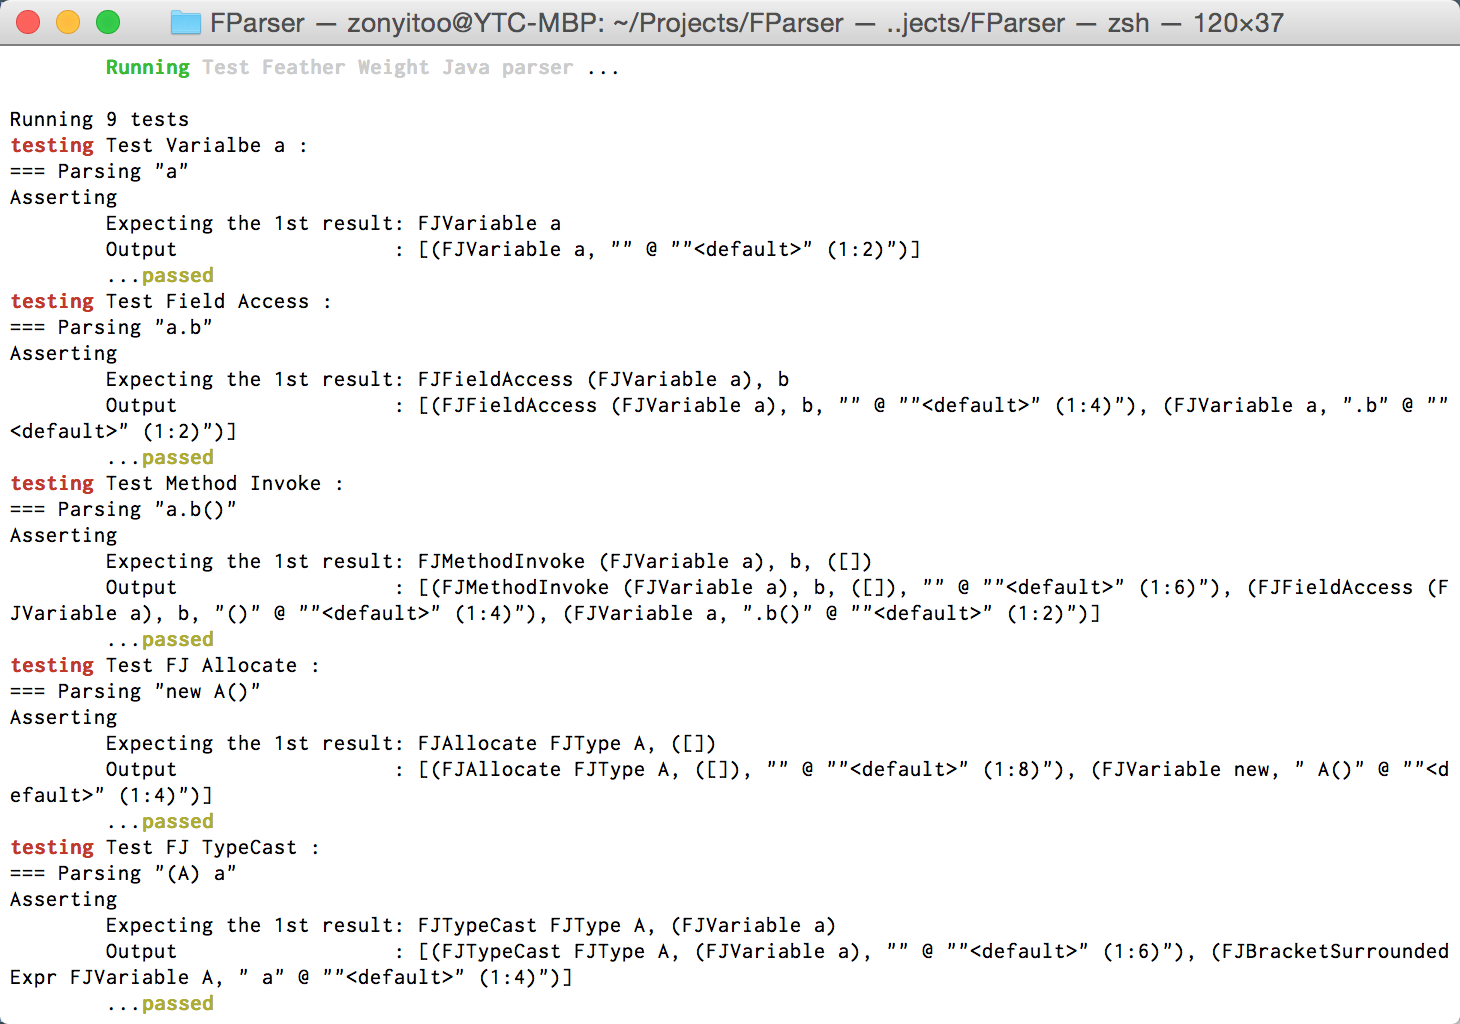
\includegraphics[width=0.8\textwidth]{imgs/Monadic_RunAllTests}
    \caption{Run all tests}
    \label{fig:monadic_runalltests}
\end{figure}
